\documentclass[11pt]{article}
\usepackage{amsmath}
\usepackage{amssymb}
\usepackage{amsthm}
\usepackage{graphicx}
\usepackage{float}

\usepackage{hyperref}
\newtheorem*{defn}{Definition}

% Roll number : 130010024 
% Name : M Suriya Kumar
\title{Mass Spring Damper}
\author{M Suriya Kumar, 130010024\thanks{This document has been prepared as part of the requirements for the first course project}}
\date{\today}
\begin{document}
\maketitle
\begin{abstract}
This document gives brief familiarity with spring mass damper system. Complete modelling and analysis of 
the system is shown. Followed by that representative simulations for various cases is also shown.
\end{abstract}
\section{Introduction}
This is one of the most widely studied topic under second order system. The system consists of a mass attached to a spring and damper. All the files
associated to this document can be found in this github repository : \url{https://github.com/msuriyak/spring-mass-damper}.

\section{Dynamics}
\begin{defn}
\hfill \break
\textbf{Linear viscous damping \cite{wiki} :} Linear damping occurs when a oscillatory variable is damped 
by an influence that opposes changes in it, in direct proportion to the instantaneous rate of change 
of the variable itself.
\end{defn}

\begin{figure}[H]
	\begin{center}
	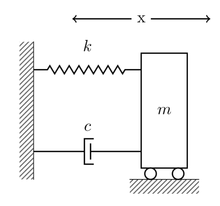
\includegraphics[scale=0.8]{spring_mass_damper.png}
	\caption{Mass attached to a spring and damper (130010024)}
	\centering
	\end{center}
\end{figure}

Mass($m$) is attached to a Hook's law spring and linear viscous damper. Say the spring constant 
is $k$ and damping coefficient of the damper is $c$.
\hfil \break
From Newton's law, 
\begin{eqnarray*}
\sum f_{ext} &=& ma, \\
\sum f_{ext} &=& f_s + f_d, \\
f_s &=& -kx, 	\\
f_d &=& -c\dot{x}, \\
-kx - c\dot{x} &=& ma, \\
ma + c\dot{x} + kx &=& 0, \\
m\ddot{x} + c\dot{x} + kx &=& 0
\end{eqnarray*}

Therefore the equation of motion is given by :
\begin{equation}
m\frac{d^2x}{dt^2} + c\frac{dx}{dt} + kx = 0
\label{eom}
\end{equation}


\section{Mass spring damper as generalized second order system}

General second-order system is given by :
\begin{equation}
\ddot{x} + 2\zeta\omega_0\dot{x} + \omega_0^2x = 0
\label{sec_ord_system}
\end{equation}
where $\zeta$ is called damping ratio and $\omega_0$ is called natural frequency.
From \ref{eom} we can get,
\begin{equation}
\ddot{x} + \frac{c}{m}\dot{x} + \frac{k}{m}x = 0
\label{mass_spring_system}
\end{equation}

Comparing coefficient with \ref{sec_ord_system}, we get
\begin{eqnarray}
\zeta &=& \frac{c}{2\sqrt{km}}, \\
\label{def_zeta}
\omega &=& \sqrt{\frac{k}{m}}
\label{def_omega}
\end{eqnarray}

\newpage
\section{State space model of the system\cite{google}}

We can describe the system only by its position and velocity. Therefore the state-space model
of the system is given by :

\[
\widetilde{x}=
\begin{bmatrix}
x \\
\dot{x}
\end{bmatrix}
\]

Therefore, equation of motion can be expressed as :
\[
\dot{\widetilde{x}}=
\begin{bmatrix}
x_2\\
- \frac{c}{m}x_2 - \frac{k}{m}x_1 + F(x_2,x_1,t)
\end{bmatrix}
\]

\section{Types of responses}

\begin{itemize}
	\item{Free response}\\
	In free response the external force is 0. That is the equation of 
	motion is given by :
	$$ \ddot{x} + \frac{c}{m}\dot{x} + \frac{k}{m}x = 0 $$

	\item{Forced/dynamic response}\\
	In forced response there exist a external force apart from spring force and 
	viscous damping force. That is the equation of motion is given by :
	$$ \ddot{x} + \frac{c}{m}\dot{x} + \frac{k}{m}x = F(\dot{x},x,t) $$

\end{itemize}


\section{Classification of system based on damping ratio}
\begin{itemize}
	\item{Under-damped system ($\zeta < 1$)}
	\item{Critically damped system ($\zeta = 1$)}
	\item{Over-damped system ($\zeta > 1$)}
\end{itemize}

\newpage
\noindent\textbf{Under-damped system :} \\
In under-damped system $\zeta$ is less than 1. \\
The free response of the system is shown in the figure below$\phantom{}_{\ref{fig1}}$.

\begin{figure}[H]
	\centering
	\centering
	\includegraphics[scale=0.5]{../output/Free_response_underdamped.png}
	\caption{Free response of a spring mass damper system (130010024)}
\end{figure}
\label{fig1}

\newpage
The forced response of the system is shown in the figure below$\phantom{}_{\ref{fig2}}$.
\begin{figure}[H]
	\centering
	\begin{tabular} {l}
	\includegraphics[width=0.8\textwidth, height=0.25\textheight]{../output/Forced_response_underdamped_under.png} \\
	\includegraphics[width=0.8\textwidth, height=0.25\textheight]{../output/Forced_response_underdamped_over.png} \\
	\includegraphics[width=0.8\textwidth, height=0.25\textheight]{../output/Forced_response_underdamped_natural.png} 
	\end{tabular}
	\caption{Forced response of a spring mass damper system (130010024)}
\end{figure}
\label{fig2}

\newpage
\noindent\textbf{Critically-damped system :} \\
In critically-damped system $\zeta$ is 1.
The free response of the system is shown in the figure below$\phantom{}_{\ref{fig10}}$.

\begin{figure}[H]
	\centering
	\centering
	\includegraphics[scale=0.5]{../output/Free_response_criticaldamped.png}
	\caption{Free response of a spring mass damper system (130010024)}
\end{figure}
\label{fig10}

\newpage
The forced response of the system is shown in the figure below$\phantom{}_{\ref{fig11}}$.

\begin{figure}[H]
	\centering
	\begin{tabular} {l}
	\includegraphics[width=0.8\textwidth, height=0.25\textheight]{../output/Forced_response_criticaldamped_under.png} \\
	\includegraphics[width=0.8\textwidth, height=0.25\textheight]{../output/Forced_response_criticaldamped_over.png} \\
	\includegraphics[width=0.8\textwidth, height=0.25\textheight]{../output/Forced_response_criticaldamped_natural.png} 
	\end{tabular}
	\caption{Forced response of a spring mass damper system (130010024)}
\end{figure}
\label{fig11}


 
\newpage
\noindent\textbf{Over-damped system :} \\
In under-damped system $\zeta$ is more than 1.
The free response of the system is shown in the figure below$\phantom{}_{\ref{fig4}}$.

\begin{figure}[H]
	\centering
	\centering
	\includegraphics[scale=0.5]{../output/Free_response_overdamped.png}
	\caption{Free response of a spring mass damper system (130010024)}
\end{figure}
\label{fig4}

\newpage
The forced response of the system is shown in the figure below$\phantom{}_{\ref{fig5}}$.

\begin{figure}[H]
	\centering
	\begin{tabular} {l}
	\includegraphics[width=0.8\textwidth, height=0.25\textheight]{../output/Forced_response_overdamped_under.png} \\
	\includegraphics[width=0.8\textwidth, height=0.25\textheight]{../output/Forced_response_overdamped_over.png} \\
	\includegraphics[width=0.8\textwidth, height=0.25\textheight]{../output/Forced_response_overdamped_natural.png} 
	\end{tabular}
	\caption{Forced response of a spring mass damper system (130010024)}
\end{figure}
\label{fig5}

\newpage
\noindent\textbf{Special case :} \\
A special case of the system arises when there is zero damping i.e $c = 0$ or $\zeta$ is zero. \\
The free response of the system is shown in the figure below$\phantom{}_{\ref{fig7}}$.

\begin{figure}[H]
	\centering
	\centering
	\includegraphics[scale=0.5]{../output/Free_response_special.png}
	\caption{Free response of a spring mass damper system (130010024)}
\end{figure}
\label{fig7}

\newpage
The forced response of the system is shown in the figure below$\phantom{}_{\ref{fig5}}$.

\begin{figure}[H]
	\centering
	\begin{tabular} {l}
	\includegraphics[width=0.8\textwidth, height=0.25\textheight]{../output/Forced_response_special_under.png} \\
	\includegraphics[width=0.8\textwidth, height=0.25\textheight]{../output/Forced_response_special_over.png} 
	\end{tabular}
	\caption{Forced response of a spring mass damper system (130010024)}
\end{figure}
\label{fig8}

\newpage
\noindent Upon forcing the system under natural frequency in this special case a resonance is observed. Under this
forcing the positon variable explodes as time goes to $\infty$.\\
Forced response is shown in the figure below$\phantom{}_{\ref{fig9}}$.


\begin{figure}[H]
	\centering
	\begin{tabular} {l}
	\includegraphics[scale=0.5]{../output/Forced_response_special_natural.png} 
	\end{tabular}
	\caption{Forced response of a spring mass damper system (130010024)}
\end{figure}
\label{fig9} 




\section{Detailed analysis of forced response\cite{norman}}

Solving the followwing equation,
$$ m\ddot{x} + c\dot{x} + kx = F(\dot{x},x,t) $$

\noindent we get 
$$ x(t) = x_p(t) + x_h(t)$$
where $x_p(t)$ is the particular solution and $x_h(t)$ is the homogeneous solution\\
\hfill \break
\noindent\textbf{Harmonic forcing :} \\
\noindent Under harmonic forcing equation of motion is given by,

\begin{eqnarray}
m\ddot{x} + c\dot{x} + kx &=& F_0cos\omega t
\end{eqnarray}
\noindent Solving for particular solution, we get
\begin{eqnarray}
x_p(t) &=& Xcos(\omega t - \phi)
\end{eqnarray}
\noindent Upon substituting particular solution in equation of motion, we get

\begin{eqnarray}
X[(k - m\omega_0^2)cos\phi + c\omega sin\phi] &=& F_0, \\ 
X[(k - m\omega_0^2)sin\phi - c\omega cos\phi] &=& 0 
\end{eqnarray}

\noindent Solving for $\phi$ and $X$, we get

\begin{eqnarray}
\phi &=& tan^{-1} \left( \frac{c\omega}{k - m\omega^2} \right), \\
\label{X}
X &=& \frac{F_0}{\sqrt{\left( k - m\omega^2\right)^2 - c^2\omega^2}}
\end{eqnarray}

\noindent Upon rearranging the terms in \ref{X}, we get 

\begin{eqnarray}
X &=& \frac{ \frac{F_0}{k} }{ \sqrt{ \left( 1 - \frac{\omega^2}{\omega_0^2} \right)^2 - \left( 2\zeta \frac{\omega}{\omega_0} \right)^2 } }, \\
\implies X &=& \frac{ \eta_{st} }{ \sqrt{ \left( 1 - r^2 \right)^2 + \left( 2\zeta r \right)^2 } } 
\end{eqnarray}

\noindent Where,
\begin{eqnarray}
\eta_{st} &=& \frac{F_0}{k}, \\
r &=& \frac{\omega}{\omega_0}
\end{eqnarray}

\noindent$\eta_{st}$ is the maximum displacement when there is a static force $F_0$ applied. \\
The ratio  of $X$ and $\eta_{st}$ is called dynamic magnifaction factor. \\
We can see that when there is no damping, dynamic magnification factor approaches $\infty$ 
when the system is forced at natural frequency. This phenomenon is called resonance. Which means 
however small the static force($F_0$), $x$ $\rightarrow$ $\infty$ as time $\rightarrow$ $\infty$
 
\bibliography{bib_file}{}
\bibliographystyle{plain}
 
\end{document}